\documentclass{report}
\title{Documentation J4K Java Library}
\author{Robin \bsc{Shin} et Thibaud \bsc{Lemaire}}
\date{PACT 2015-2016}

\usepackage[latin1]{inputenc}
\usepackage[T1]{fontenc}
\usepackage[francais]{babel}
\usepackage{graphicx}
\usepackage[top=2cm, bottom=2cm, left=2cm, right=3cm]{geometry}
\usepackage{verbatim}

\begin{document}
\maketitle
\chapter*{Installation}

Tout d'abord, il est \textit{imp\'eratif} d'avoir la version 1.8 du SDK Kinect et non la 2.0 car celle-ci est inexploitable (probl\`emes de pilotes).

\subsection*{T\'el\'echargement du fichier .jar}
Sur : \underline{http://research.dwi.ufl.edu/ufdw/download.php}, t\'el\'echarger ufdw.jar.

\subsubsection*{Int\'egration avec Eclipse}
\begin{enumerate}
\item Ouvrir Eclipse, aller dans Project > Properties et aller dans l'onglet Java Build Path
\item Cliquer sur le bouton "Add External JARs..." et choisir le chemin vers le fichier ufdw.jar pr\'ec\'edemment t\'el\'echarg\'e.
\item D\'eplacer le fichier "ufdw\_j4k\_32bit.dll" ou "ufdw\_j4k\_64bit.dll" en fonction de la machine utilis\'ee \`a la racine du projet Java pour \'eviter les probl\`emes de dll manquantes.
\item On peut d\'esormais importer les fichiers de la librairie gr?ce ? la commande "import edu.ufl.digitalworlds.j4k.*".
\end{enumerate}

\subsubsection*{Recommandations pour l'int\'egration avec git}
\begin{enumerate}
\item Tout d'abord, il ne faut surtout pas ignorer le fichier .classpath au risque d'avoir des probl\`emes avec git.
\item Dans le fichier .classpath, le chemin vers ufdw.jar doit ?tre relatif et non absolu au risque de conflits d\`es qu'un utilisateur souhaite faire un push ou un pull.
\end{enumerate}

\subsubsection*{Ajout d'un projet de d\'emonstration sous Eclipse}
\begin{enumerate}
\item Ouvrir Eclipse, aller dans File > Import... et s\'electionner Git > Projects from Git
\item S\'electionner URI puis cliquer sur "Next"
\item Copier \underline{http://research.dwi.ufl.edu/git/j4kdemo} dans l'espace d\'edi\'e ? l'URI et cliquer sur "Next" autant de fois que n\'ecessaire, puis "Finish" : un nouveau projet "j4kdemo" est cr\'ee.
\end{enumerate}



\chapter*{Cr\'eation de l'objet Kinect}
\section*{Initialisation}
\verb"public int start(int flags);"

Initialise la Kinect, les donn\'ees, le squelette, etc... L'entier flags pass\'e en param\`etre permet d'ajouter des options, en fonction des besoins du projet. Par exemple, \verb"flag = COLOR" initialise la Kinect avec une image en couleur,  \verb"DEPTH" permet d'avoir la 3D et \verb"flag = SKELETON" permet d'exploiter le squelette. On peut enfin cumuler ces options gr\^ace au s\'eparateur \verb"|".


\section*{M\'ethodes}
\verb"public void onSkeletonFrameEvent(boolean[] skeleton_tracked, float[] positions, float[] orientations,"
\newline
\verb"byte[] joint_status);"

M\'ethode appel\'ee lorsqu'un nouveau squelette est re\c{c}u. Cette m\'ethode remplace le squelette de l'attribut associ\'e de type Skeleton, cr\'ee un \'ev\'enement et l'envoie \`a tous les modules via un syst\`eme de Listeners.

Il est important d'exploiter le tableau de bool\'eens \verb"skeleton_tracked" pour savoir quel squelette a \'et\'e re\c{c}u sous peine d'un comportement de la Kinect assez impr\'evisible.

\hspace{1\baselineskip}

\verb"public void onDepthFrameEvent(short[] arg0, byte[] arg1, float[] arg2, float[] arg3);"

Cette m\'ethode est appel\'e lorsque le depthFrame est recu.
      
      
\hspace{1\baselineskip}

\verb"public void stop();"

Cette m\'ethode permet d'arr\^eter la Kinect et de fermer le flux pr\'ec\'edemment ouvert.


\chapter*{Comment les \'ev\'enements sont-ils r\'ecup\'er\'es?}
Les \'ev\'enements sont r\'ecup\'er\'es via un syst\`eme de Listeners.

\section*{Qu'est-ce qu'un listener?}
Un listener est une instance d'une classe qui poss�des certaines m�thodes qui sont destin�es � �tre appel�es par un gestionnaire d'�v�nement. Une classe de listener doit h\'eriter de la classe 'EventListener'. Nous allons nous servir de ces listeners pour faire les transitions entre tous les modules de notre projet.

\section*{Utilisation dans notre projet}

\subsection*{La classe KinectEvent}
Nous avons besoin de cr\'eer une nouvelle classe KinectEvent. En effet, ce sera un objet de la classe KinectEvent qui sera r\'ecup\'er\'e par les autres modules. Cette classe poss\`ede un attribut Skeleton et un attribut long repr\'esentant le temps. Elle poss\`ede \'egalement deux getters permettant de r\'ecup\'erer ces attributs, et permettant ainsi \`a la classe ayant re\c{c}u un \'ev\'enement d'exploiter le squelette.

\subsection*{L'interface KinectListenerInterface}
Cette interface va \^etre impl\'ement\'ee par toutes les classes ayant besoin d'\'ecouter la classe Kinect. Cette interface ne contient qu'une m\'ethode de signature \verb"void skeletonReceived(KinectEventInterface e);" qui va devoir \^etre impl\'ement\'ee \`a chaque fois qu'une classe impl\'emente KinectListenerInterface. C'est cette m\'ethode qui sera appel\'ee d\`es qu'un KinectEventInterface sera re\c{c}u.


\newpage
\chapter*{Comment le squelette est-il manipul\'e?}
On suppose avoir un objet de type Skeleton appel\'e squelette. Alors la classe Skeleton impl\'ement\'ee par la J4KSDK fournit directement des m\'ethodes de signatures \verb"public float get3DJointX(int joint_id);", \verb"public float get3DJointY(int joint_id);", \verb"public float get3DJointZ(int joint_id);" permettant de r\'ecup\'erer respectivement les coordonn\'ees $(x, y, z)$ du squelette. Enfin, la classe Skeleton contient plusieurs constantes de classes permettant de tracker une partie du corps bien pr\'ecise en rempla\c{c}ant l'entier \verb"joint_id" par une des constantes de classes suivantes :

\hspace{1\baselineskip}

\begin{center}
\begin{tabular}{|c|c|c|}
\hline
Identifiant & Entier associ\'e \\
\hline
SPINE\_BASE & 0 \\
\hline
SPINE\_MID & 1 \\
\hline
NECK & 2 \\
\hline
HEAD & 3 \\
\hline
SHOULDER\_LEFT & 4 \\
\hline
ELBOW\_LEFT & 5 \\
\hline
WRIST\_LEFT & 6 \\
\hline
HAND\_LEFT & 7 \\
\hline
SHOULDER\_RIGHT & 8 \\
\hline
ELBOW\_RIGHT & 9 \\
\hline
WRIST\_RIGHT & 10 \\
\hline
HAND\_RIGHT & 11 \\
\hline
HIP\_LEFT & 12 \\
\hline
KNEE\_LEFT & 13 \\
\hline
ANKLE\_LEFT & 14 \\
\hline
FOOT\_LEFT & 15 \\
\hline
HIP\_RIGHT & 16 \\
\hline
KNEE\_RIGHT & 17 \\
\hline
ANKLE\_RIGHT & 18 \\
\hline
FOOT\_RIGHT & 19 \\
\hline
SPINE\_SHOULDER & 20 \\
\hline�
HAND\_TIP\_LEFT & 21 \\
\hline
THUMB\_LEFT & 22 \\
\hline
HAND\_TIP\_RIGHT & 23 \\
\hline
THUMB\_RIGHT & 24 \\
\hline
JOINT\_COUNT & 25 \\
\hline
\end{tabular}
\end{center}

\section*{Exemple pour tracker la main droite}
Il suffit de tapper les lignes de commandes : 
\newline
\verb"int x, y, z;"
\newline
\verb"x = get3DJointX(Skeleton.HAND_RIGHT);"
\newline
\verb"y = get3DJointY(Skeleton.HAND_RIGHT);"
\newline
\verb"z = get3DJointZ(Skeleton.HAND_RIGHT);"

Alors les coordonn\'ees de la main droite sont $(x, y, z)$.


\chapter*{Annexe : Utilisation de Kinect Studio}
T\'el\'echarger et installer tout d'abord Kinect Studio, inclus dans Kinect Windows Developer Toolkit v1.8 (lien : \underline{https://www.microsoft.com/en-us/download/details.aspx?id=40276}).

\begin{enumerate}
\item Lancer Kinect Studio
\item Une fen\^etre s'ouvre, demandant de lancer la Kinect. Brancher la Kinect en USB et lancer le programme Java (qui doit contenir la ligne de commande \verb"start(int flag);", en rempla\c{c}ant l'entier flag).
\item Appuyer sur "Refresh" : la Kinect apparait. Cliquer sur "Connect".
\item Aller dans View > Color, Depth ou 3D View pour afficher la vue de la Kinect (attention : pour afficher la vue en couleur, le param\`etre \verb"flag" dans la m\'ethode \verb"start" doit contenir \verb"J4KSDK.COLOR". De m\^eme pour la vue en profondeur).
\end{enumerate}

On peut alors enregistrer une s\'equence en appuyant sur le bouton "Record", arr\^eter l'enregistrement en appuyant sur "Stop" et la rejouer avec "Play/Pause". Il est \'egalement possible d'ouvrir un enregistrement (de type Kinect Studio Files) et de le rejouer.

\begin{figure}[h!]
\centering
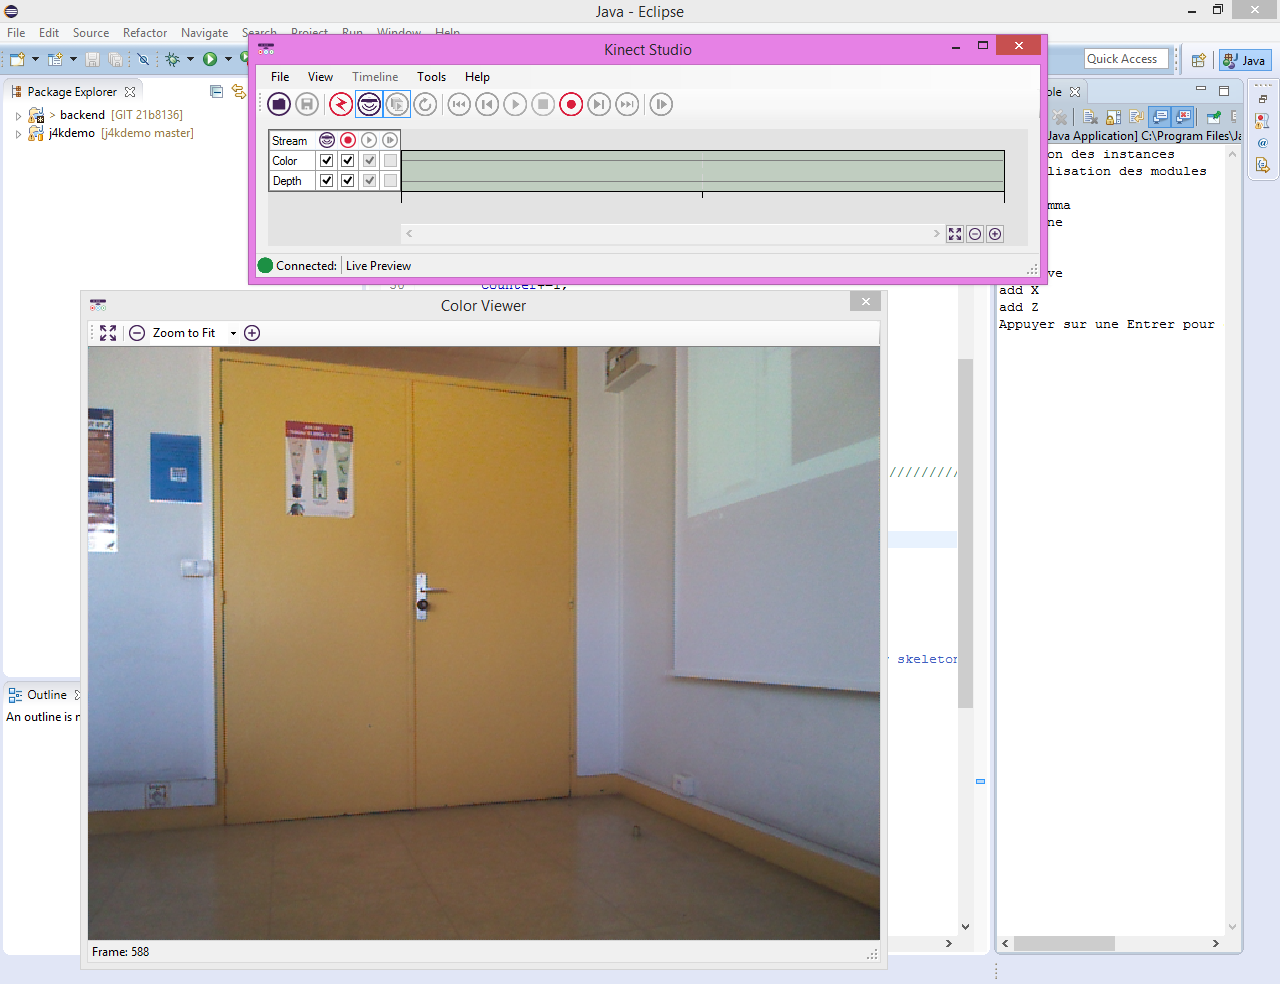
\includegraphics[height=4in]{Images/KinectStudio.png}
\caption{Kinect Studio et l'affichage de la vue en couleur.}
\end{figure}


















\end{document}